\section{Neural Networks}
\begin{frame}{\insertsec}
	\def\layersep{2.5cm}

\begin{figure}[H]
    \centering
    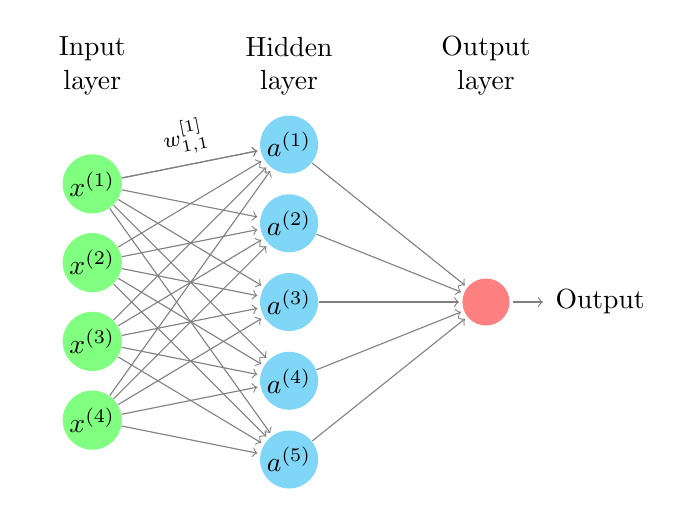
\begin{tikzpicture}[shorten >=1pt,->,draw=black!50, node distance=\layersep]
        \tikzstyle{every pin edge}=[<-,shorten <=1pt]
        \tikzstyle{neuron}=[circle,fill=black!25,minimum size=17pt,inner sep=1pt]
        \tikzstyle{input neuron}=[neuron, fill=green!50];
        \tikzstyle{output neuron}=[neuron, fill=red!50];
        \tikzstyle{hidden neuron}=[neuron, fill=cyan!50];
        \tikzstyle{annot} = [text width=4em, text centered]
        
        % Draw the input layer nodes
        \foreach \y in {1,...,4} {
            % This is the same as writing \foreach \name / \y in {1/1,2/2,3/3,4/4}
            \node[input neuron] (I-\y) at (0,-\y) {$x^{(\y)}$};
        }
        % Draw the hidden layer nodes
        \foreach \y in {1,...,5} {
            \node[hidden neuron, yshift=.5cm] (H-\y) at (\layersep,-\y cm) {$a^{(\y)}$};
        }
        
        % Draw the output layer node
        \node[output neuron,pin={[pin edge={->}]right:Output}, right of=H-3] (O) {};
        
        % Connect every node in the input layer with every node in the
        % hidden layer.
        \foreach \source in {1,...,4}
            \foreach \dest in {1,...,5}
                \path (I-\source) edge (H-\dest);
        
        \path (I-1) edge node[sloped, above] {\footnotesize  $w_{1, 1}^{[1]}$} (H-1);
        
        % Connect every node in the hidden layer with the output layer
        \foreach \source in {1,...,5}
            \path (H-\source) edge (O);
        
        % Annotate the layers
        \node[annot,above of=H-1, node distance=1cm] (hl) {Hidden layer};
        \node[annot,left of=hl] {Input layer};
        \node[annot,right of=hl] {Output layer};
    \end{tikzpicture}
    \caption{Representation of Neural Network}
\end{figure}

\end{frame}

\subsection{Parameters}
\begin{frame}{\insertsubsec}
    \begin{columns}[t]
        \column{.6\textwidth}
        \begin{itemize}
            \item $l$: Current layer
            \item $w_{i, j}^{[l]}$: Weight from unit $j$ to $i$ at layer $l$
            \item $b_{i}^{[l]}$: Bias for unit $i$ at layer $l$
            \item $n^{[l]}$: Number of units in layer $l$
            \item $W^{[l]} \in \mathbb{R}^{n^{[l]} \times n^{[l - 1]}}$: Weight matrix
            \item $\bm{b}^{[l]} \in \mathbb{R}^{n^{[l]}}$: Bias
            \item $
            \begin{aligned}[t]
                \bm{a}^{[l]} &= g(W^{[l]}\cdot \bm{a}^{[l - 1]} + \bm{b}^{[l]}) \\
                \bm{a}^{[l]} &\in \mathbb{R}^{n^{[l]}}
            \end{aligned}
            $ Activations for layer $l$
            \item $g(x)$: Activation function
        \end{itemize}
        \column{.5\textwidth}
        \centering
        \begin{columns}[t]
    \column{.5\textwidth}
    \centering
    \begin{figure}
        \begin{tikzpicture}
            \begin{axis}[
                width=\textwidth,
                height=.8\textwidth,
                grid=major,
                grid style={dashed, gray!30},
                xtick={-5, 0, 5},
                xticklabels={$-\infty$, $0$, $+\infty$}
                ]
                \addplot[mark=none]{tanh(x)};
            \end{axis}
        \end{tikzpicture}
        \caption{$\tanh(x)$}
    \end{figure}
    \centering
    \column{.5\textwidth}
    \begin{figure}
        \begin{tikzpicture}
            \begin{axis}[
                width=\textwidth,
                height=.8\textwidth,
                grid=major,
                grid style={dashed, gray!30},
                xtick={-5, 0, 5},
                xticklabels={\empty, $0$, \empty}
                ]
                \addplot[mark=none]{max(x, 0)};
            \end{axis}
        \end{tikzpicture}
        \caption{ReLU function}
    \end{figure}
\end{columns}
    \end{columns}
\end{frame}
\begin{frame}
    \begin{columns}
        \column{.6\textwidth}
        \begin{block}{Cost function}
            $$
            J(\bm{W}, \bm{b}, \hat{\bm{y}}, \bm{y}) = 
            \frac{1}{m} \sum_{i=1}^{m} \mathcal{L}(\hat{\bm{y}}^{(i)}, \bm{y}^{(i)})
            $$
        \end{block}
        \begin{block}{Loss function}
            $$
            \mathcal{L}(\hat{\bm{y}}, \bm{y}) = ||\hat{\bm{y}} - \bm{y}||^2
            $$
        \end{block}
        \begin{block}{Parameters update}
            \begin{align*}
            W^{[l]} &:= W^{[l]} - \alpha \cdot \frac{\partial J}{\partial W^{[l]}} \\
            \bm{b}^{[l]} &:= \bm{b}^{[l]} - \alpha \cdot \frac{\partial J}{\partial \bm{b}^{[l]}}
            \end{align*}
        \end{block}
        \column{.4\textwidth}
        To achieve better results at predicting $\hat{\bm{y}}$ 
        we have to minimize the cost function $J(\bm{W}, \bm{b}, \hat{\bm{y}}, \bm{y})$.
    \end{columns}
\end{frame}

\subsection{Regularization}
\begin{frame}{\insertsubsec}
    To prevent overfitting add the weights to the cost function so we also try to minimize
    big weights.

    \begin{align*}
        J(\bm{W}, \bm{b}, \hat{\bm{y}}, \bm{y}) &= 
        \frac{1}{m} \sum_{i = 1}^m \mathcal{L}(\hat{\bm{y}}, \bm{y}) + 
        \frac{\lambda}{2m} \sum_{l=1}^L ||W^{[l]}||^2_F \\ 
        \underbrace{||W^{[l]}||^2_F}_{\text{Frobenius Norm}} &= \sum_i \sum_j (w_{ij}^{[l]}) \\ 
        dW^{[l]} &= \text{from backprop } + \frac{\lambda}{m} \cdot W^{[l]} \\
        \lambda &\rightarrow \text{Regularization parameter}
    \end{align*}

    It cancels some effects from some units creating a simple model.
\end{frame}
\begin{frame}[fragile]{Dropout Regularization}
    Go through each layer of the network and set some probability of elimination for each unit. 
    This is done for \textbf{each sample}.

    \begin{figure}
        \begin{verbatim}
drop = np.random.randn(*a_prev.shape) < keep_prob
a_next = np.multiply(a_prev, drop)
a_next /= keep_prob
        \end{verbatim}
        \caption{Example using \texttt{numpy}}
    \end{figure}

    \begin{alertblock}{Predictions during test time}
        No dropout is used during test time since it wouldn't make sense.
    \end{alertblock}
\end{frame}

\begin{frame}{Adam optimization algorithm}
    Training a NN is a minimization problem. In this case we always use gradient descent
    to find the minimum. Sometimes the gradient can go too fast.

    \begin{onlyenv}<1>
        \begin{align*}
            V_{dW} &= \beta_1 V_{dW} + (1 - \beta_1) \cdot dW \\
            S_{dW} &= \beta_2 S_{dW} + (1 - \beta_2) \cdot dW^2 \\
            W &:= W - \alpha \cdot \frac{V_{dW}}{\sqrt{S_{dW}} + \varepsilon}
        \end{align*}
    \end{onlyenv}
    \begin{onlyenv}<2>
        
\begin{figure}[H]
    \begin{tikzpicture}
\begin{axis}[
        width=.9\textwidth,
        height=.6\textwidth,
        xlabel=Day,
        ylabel={T $(^{\circ}C)$},
        every axis y label/.style={at={(current axis.north west)},above=2mm},
        ymax = 45,legend style={font=\fontsize{4}{5}\selectfont},
        clip marker paths=true
    ]
    \addplot[
        mark=*,
        mark size=1,
        draw=cyan!50
    ] table[
        x index = 0, 
        y index = 1, 
        header=true, 
        col sep = comma, 
        only marks
    ]{drawings/daily_temperature.csv};
    \addlegendentry{Data}
    \addplot[
        mark=none,
        draw=red!50,
        thick
    ] table[
        x index = 0, 
        y index = 2, 
        header=true, 
        col sep = comma
    ]{drawings/daily_temperature.csv};
    \addlegendentry{$\beta = .99$}
    \addplot[
        mark=none,
        draw=violet,
        thick
    ] table[
        x index = 0, 
        y index = 4, 
        header=true, 
        col sep = comma
    ]{drawings/daily_temperature.csv};
    \addlegendentry{$\beta = .90$}
\end{axis}
    \end{tikzpicture}
    
\end{figure}



    \end{onlyenv}
\end{frame}

\subsection{Hyper-parameters}
\begin{frame}{\insertsubsec}
    \begin{itemize}
        \item $m$: Mini-batch size
        \begin{itemize}
            \item $m = 1$: Stochastic gradient descent
            \item $m = $ set size: Batch gradient descent
        \end{itemize}
        \item $\alpha$: Learning rate
        \begin{itemize}
            \item Learning rate decay 
            $\alpha = \frac{1}{1 + \text{decay-rate}\times \text{epoch}} \cdot \alpha_0$
            \item Exponential decay
            $\alpha = 0.95^{\alpha_0}$

        \end{itemize}
        \item $L$: Number of layers
        \item Number of iterations
        \item Number of hidden units
    \end{itemize}
\end{frame}
